\section{Computational Dialog Modeling}
\textcolor{red}{MISSING LECTURE 10 (what should we put in here at all?)}
\subsection{Modular dialog systems}
\begin{itemize}
	\item There are two main tasks in dialog modeling: either understand a conversation from outsider's view (summarizing), or the capability to take part in conversation $\Rightarrow$ make a dialog agent
	\item First approaches of modeling dialog agent were based on hand-specified patterns/transformation rules based on keywords to find an appropriate answer
	\item Recently, the focus shifted towards data-driven methods by either retrieving existing information or generating new sentences by i.e. Encoder-Decoder architectures
	\item Problems: hard to evaluate, such systems often show to just copy patterns in training dataset but don't generalize well.
	\item Different approach: in dialogs, there is a tendency to ascribe goal and \textbf{intentions}
	\item However, intentions are not easy to recognize. That's why such methods are often used for \textbf{task-oriented} dialog systems where the end-goal makes intentions tractable
	\item The modular dialog system architecture: 
	\begin{figure}[ht]
		\centering
		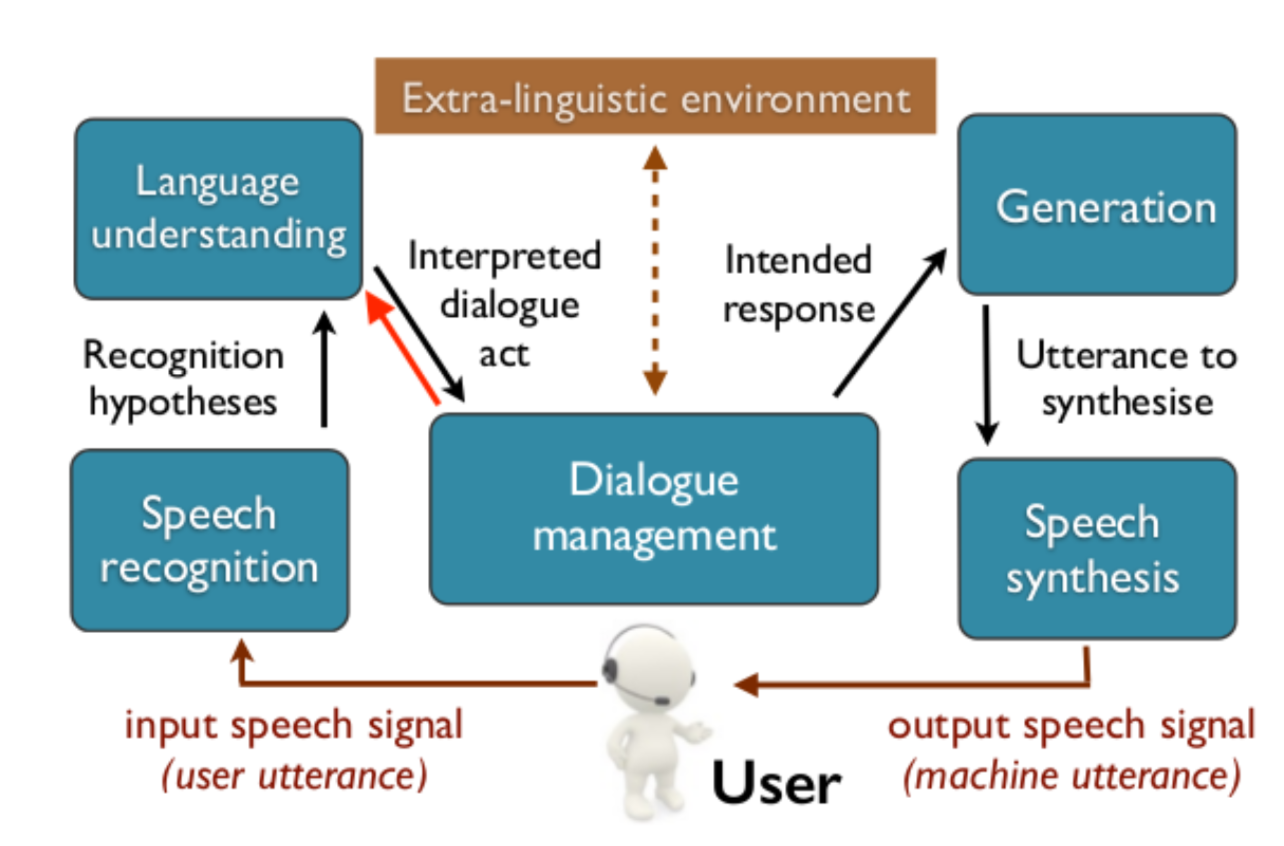
\includegraphics[width=0.4\textwidth]{figures/dialog_modeling_modules.png}
	\end{figure}
	\item \textit{Language understanding}: NLP1 course. Morphology, POS tagging, lexical semantics and syntactic parsing, compositional semantics, ...
	\item \textit{Dialog management}: consists of two modules:
	\begin{itemize}
		\item \textit{Dialog state tracker}: handle linguistic context (what has been said) and how relevant it is to the task. We can convert messages into slots with parameters (like \texttt{request(name)}) to simplify the task. 
		\item \textit{Dialog policy}: select what action to take next/model the next answer. Estimate probabilities for possible actions, and choose best ones. Training mostly done in a reinforcement learning way with simulator
	\end{itemize}
	\item \textit{Extra-linguistic environment}: taking information into account which is not coming from this dialog itself (images, databases, ...)
\end{itemize}
\subsection{Visually grounded, task-oriented dialog}
\begin{itemize}
	\item \textbf{Visual dialog}: given an image and a history of human-dialog, answer a follow-up question 
	\item We can evaluate this task with the same metrics as for summarization and translation (BLEU, ROGUE)
	\item However, in this task the agent is thrown at random into a conversation without being able to interact
	\item \textit{Image guessing game}: one agents ($Q$) sees the original image, and the other agent ($A$) sees the image with the object highlighted that $Q$ needs to guess
	\item Current implementation is based on LSTMs with CNN encoders. Still, the models perform poorly compared to humans
\end{itemize}